\section*{Administrative}

\begin{frame}
    \frametitle{Logistics}
    \begin{description}
        \item[Lecture times:] 
        \begin{itemize}
        \item Lecture Monday, 12:30, room 25.13.U1.32
        \item Lecture Wednesday, 12:30, room 24.21.00.61
        \item Tutorial Tuesday, 12:30, room 25.22.U1.74
        \end{itemize}
    \item[Email:] \href{paul.swoboda@hhu.de}{paul.swoboda@hhu.de}
    \item[Discord Server:] : \href{https://discord.gg/pyEdkHTpm}{https://discord.gg/pyEdkHTpm}
    \item[Lecture Materials:] Will be posted on discord.
    \pause 
    \item[Grading:] 
    \begin{itemize}
        \item Exercise sheets: 
        \begin{itemize}
            \item Each one or two weeks a sheet will be given out.
            \item You have to obtain at least 50\% of the points to be admitted to the exam.
        \end{itemize}
        \pause \item Exam: A final written or oral exam, depending on the number of participants.
        \pause \item Grade: Exercise sheets and exam contribute half to the final grade each.
    \end{itemize}
    \end{description}
\end{frame}

\begin{frame}{Lecture Flavour}
    \begin{itemize}
    \item Theoretically challenging: 
    \begin{itemize}
        \item Interesting and advanced probabilistic techniques will be discussed.
        \pause \item Algorithms are intricate (but beautiful).
    \end{itemize}
    \pause \item Practically oriented:
    \begin{itemize}
        \item Programming will be done in python.
    \pause \item In the first part of the lecture we will be reimplementing some classical inference/learning algorithms for graphical models.
    \pause \item In the second part we will dive deeper into deep generative models using pytorch.
    \end{itemize}
    \pause \item Prerequisites:
    \begin{itemize}
    \item Machine Learning: Training, errors, losses, prediction, classification, $\ldots$
    \pause \item Deep Learning: NNs and their architecture, training with backprop and gradient descent, coding them, $\ldots$
    \pause \item Probability: Random variables, distributions, expectations and their conditional variants
    \pause \item Graph theory: Basic concepts like nodes, directed arcs and undirected edges, cliques, cycles, $\ldots$
    \pause \item Optimization and analysis: Gradients, Jacobians, gradient descent, chain rule, $\ldots$
    \end{itemize}
    \pause \item A few words before:
    \begin{itemize}
        \pause \item Lecture will be slow-moving: We will discuss a limited amount of content in depth
    \pause \item You will become a probability distribution ninja!
    \pause \item Ask questions! Almost no question is too stupid.
    \pause \item Initiate discussions! If discussion is too stupid, I will stop it.
    \item People who do not like formulas and proofs will suffer
        \begin{itemize}
        \pause \item We will go through each formula in detail for deep understanding.
        \end{itemize}
    \end{itemize}
    \pause \item \textcolor{red}{Lecture will be work-intensive!} Sorry, but ML is like that.
\end{itemize}
\vspace{-1.9cm}
\hfill

\includegraphics[height=1.8cm]{img/must_work_hard.jpeg}
\end{frame}

\begin{frame}
    \frametitle{Materials}
\begin{description}
    \item[Slides:] Will be posted on discord.
    \begin{itemize}
    \item Please post bugs/errors you find in discord as well!
    \end{itemize}
\item[Textbooks:] Can be (partly) found online and include
\begin{itemize}
\item Daphne Koller and Nir Friedman, Probabilistic Graphical Models
\item M.\ I.\ Jordan, An Introduction to Probabilistic Graphical Models
\item Kevin P.\ Murphy: Probabilistic Machine Learning: Advanced Topics
\item David MacKay: Information Theory, Inference, and Learning Algorithms
\item Steffen L.\ Lauritzen: Graphical Models
\end{itemize}
\item[Lecture notes:]
\begin{itemize}
\item \href{https://ermongroup.github.io/cs228/}{CS 228 Stanford, Stefano Ermon}
\item \href{https://cedar.buffalo.edu/~srihari/CSE674/}{CSE 647 Buffalo, Sargur Srihari}
\item \href{https://cedar.buffalo.edu/~srihari/CSE674/}{10-708 CMU, Eric Xing}
\end{itemize}
\item[Papers:]
\begin{itemize}
\item I will reference important research and good overview papers as we go.
\item You should be able to read research papers yourself after completing the course!
\end{itemize}
\end{description}
\end{frame}

\section{Introduction}

\begin{frame}{PML Rationale: Discriminative vs.\ Generative}
    \begin{itemize}
    \item What do you care about in deep learning? 
    \begin{itemize}
        \pause \item Classification/regression accuracy.
        \pause \item Good features.
    \pause \item Discriminative machine learning!
    \end{itemize}
    \pause \item If you want to generate new data, what would be needed? 
    \begin{itemize}
        \pause \item Mathematical option: Sampling from a probability distribution.
    \pause \item Generative machine learning!
    \end{itemize}
    \pause \item But: Probability distribution over e.g.\ images? 
    \begin{itemize}
        \pause \item Directly learning/sampling distribution is impossible!
        \pause \item $512 \times 512 \times 3$ dimensional image, $256$ intensity values \pause $\rightarrow$ $255^{786,432}$ states!
    \end{itemize}
\end{itemize}
\begin{center}

\pause 
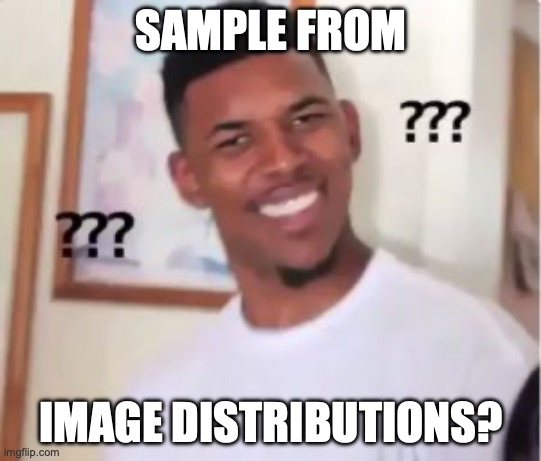
\includegraphics[width=0.35\textwidth]{img/sample_from_image_distributions.jpeg}
\end{center}
\end{frame}
%
\begin{frame}{PML Rationale: Deterministic vs.\ Probabilistic}
    \begin{itemize}
    \pause \item Classical AI: Reason by designing/learning hard rules, planning \& infering solutions 
    \begin{itemize}
        \pause \item \textbf{Problem:} does not work in real world!
    \end{itemize}
    \pause \item Reason with uncertainty: Probabilistic graphical models et al.
    \begin{itemize}
    \pause \item Learn uncertainties from data, do not hand-design things!
    \end{itemize}
\end{itemize}
\begin{center}
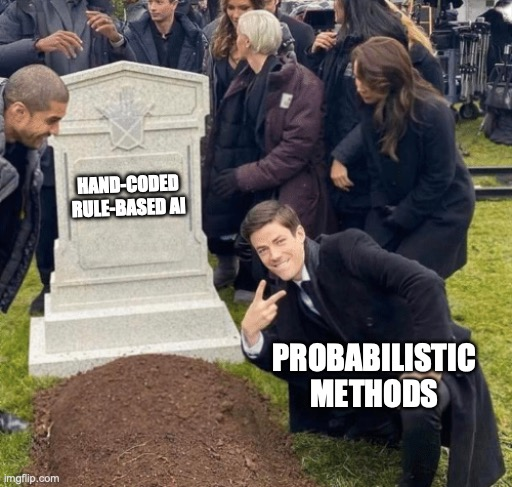
\includegraphics[width=0.4\textwidth]{img/prob_cs_classical_ai.jpeg}
\end{center}
\end{frame}
%
\begin{frame}{PML Rationale: Structure \& Sparsity}
\begin{itemize}
\item Brain has $10^{11}$ neurons and $10^{14}$ synapses \pause $\Rightarrow$ sparsely connected!
\pause \item Probabilistic machine learning achieves tractability by restricting interactions in distributions.
\begin{itemize}
\pause \item Conditional independence in distributions $\Leftrightarrow$ sparse connections between variables.
\pause \item Sparsely composing simple building blocks to obtain complicated distributions.
\end{itemize}
\end{itemize}
\pause
\begin{center}

\includegraphics[width=0.4\textwidth]{img/sparse_connections.jpeg}
\end{center}
\end{frame}

\subsection*{Probabilistic Graphical Models}
\begin{frame}
    \frametitle{Probabilistic Concepts}
\begin{description}
\item[Representation:] Probability distributions of multiple variables:
 \begin{equation}
 \Pb[X_1,X_2,\ldots,X_n], \quad X_i \in L_i
 \end{equation}
 \begin{itemize}
    \item Assume $L_i = \{0,1\}$ for all $i$. How many possible values can $\Pb$ attain? \pause $2^n$.
    \pause \item Are they all needed for representing $\Pb$ in real-world scenarios?
    \pause \item Would a full representation give us insights/interpretation?
    \pause \item How can we effectively represent high-dimensional distributions?
    \item How can we input prior knowledge?
\end{itemize}
\pause
\item[Learning:] How to get all values for computing $\Pb$?
\begin{itemize}
    \pause \item Maximum likelihood estimation (MLE)? How many data points would we need?
\pause \item Other estimation approaches? \pause What to do when not all values are observed?
\end{itemize}
\pause \item[Inference:] 
\begin{itemize}
    \item How do we sample from the distribution? 
    \pause \item How do we compute conditional probabilities?
    \pause \item When a subset of variables has been observed, what is the distribution of the unobserved (hidden) variables?
    \pause \item Computing $\Pb[X_{hidden}|X_{obs}] = \frac{\Pb[X]}{\sum_{X' : X'_{obs} = X_{obs}} \Pb[X']}$ (also called querying/marginalization) requires evaluating $\abs{L}^{\abs{hidden}}$ variables. \pause Not tractable!
\end{itemize}
\end{description}
\end{frame}

\begin{frame}
    \frametitle{Probabilistic Graphical Models (PGM)}
    \begin{columns}[t]
    \column{0.5\textwidth}
\begin{itemize}
\item A PGM is a graph representing relationship among individual random variables.
\begin{itemize}
    \item Node: Random Variable
    \item Edge/arc: Relationship for pairs of random variables.
    \item No edge/arc: Absence of $\ldots$
\end{itemize}
\pause
\item What could a relationship between variables be?
\begin{itemize}
\pause \item Correlation/Independence?
\pause \item Conditional Correlation/Independence?
\pause \item Causality?
\end{itemize}
\end{itemize}

\pause

\textbf{Example Correlation\footnotemark[1]:} Let 
\begin{itemize}
\item $X$: height of a child
\item $Y$: vocabulary of a child
\item $Z$: age of a child
\end{itemize}
\begin{center}
    \begin{tikzpicture}[scale=0.2,baseline=(b.base)]
            \node (b) at (0,-0.5) {};
            \node [style=rand_var] (0) at (-2, 1) {$Y$};
            \node [style=rand_var] (1) at (2, 1) {$X$};
            \node [style=rand_var] (2) at (0, -2) {$Z$};
            \draw (0) to (1);
            \draw (2) to (1);
            \draw (0) to (2);
    \end{tikzpicture}
    \hspace{0.3cm} vs.\ \hspace{0.3cm}
    \begin{tikzpicture}[scale=0.2,baseline=(b.base)]
            \node (b) at (0,-0.5) {};
            \node [style=rand_var] (0) at (-2, 1) {$Y$};
            \node [style=rand_var] (1) at (2, 1) {$X$};
            \node [style=rand_var] (2) at (0, -2) {$Z$};
            \draw (2) to (1);
            \draw (0) to (2);
    \end{tikzpicture}
\end{center}
    \column{0.5\textwidth}
\pause
\textbf{Example Causality:} Let
\begin{itemize}
    \item $X$: going to heaven
    \item $Y$: being  virtuous
    \item $Z$: having the right faith
    \end{itemize}
    \begin{center}
        \begin{tikzpicture}[scale=0.2,baseline=(b.base)]
            \node (b) at (0,-0.5) {};
                \node [style=rand_var] (Y) at (-2, 1) {$Y$};
                \node [style=rand_var] (X) at (2, 1) {$X$};
                \node [style=rand_var] (Z) at (0, -2) {$Z$};
                \draw[->] (Y) to (X);
                \draw[->] (Z) to (X);
        \end{tikzpicture}
       \hspace{0.1cm} vs \hspace{0.1cm}
       \begin{tikzpicture}[scale=0.2,baseline=(b.base)]
            \node (b) at (0,-0.5) {};
            \node [style=rand_var] (Y) at (-2, 1) {$Y$};
            \node [style=rand_var] (X) at (2, 1) {$X$};
            \node [style=rand_var] (Z) at (0, -2) {$Z$};
            \draw[->] (Y) to (X);
            \draw[->] (Z) to (X);
            \draw[->] (Z) to (Y);
       \end{tikzpicture} 
       \hspace{0.1cm} vs \hspace{0.1cm}
       \begin{tikzpicture}[scale=0.2,baseline=(b.base)]
            \node (b) at (0,-0.5) {};
        \node [style=rand_var] (Y) at (-2, 1) {$Y$};
        \node [style=rand_var] (X) at (2, 1) {$X$};
        \node [style=rand_var] (Z) at (0, -2) {$Z$};
        \draw[->] (Z) to (X);
\end{tikzpicture} 
    \end{center}
\pause
\textbf{Example Independence\footnotemark[1]:} Let
\begin{itemize}
    \item $X$: IQ
    \item $Y$: Genetics
    \item $Z$: Social factors
    \end{itemize}
    \begin{center}
       \begin{tikzpicture}[scale=0.2,baseline=(b.base)]
            \node (b) at (0,-0.5) {};
                    \node [style=rand_var] (Y) at (-2, 1) {$Y$};
                    \node [style=rand_var] (X) at (2, 1) {$X$};
                    \node [style=rand_var] (Z) at (0, -2) {$Z$};
                    \draw[->] (Y) to (Z);
                    \draw[->] (Z) to (X);
            \end{tikzpicture} 
       \hspace{0.1cm} vs \hspace{0.1cm}
       \begin{tikzpicture}[scale=0.2,baseline=(b.base)]
            \node (b) at (0,-0.5) {};
                \node [style=rand_var] (Y) at (-2, 1) {$Y$};
                \node [style=rand_var] (X) at (2, 1) {$X$};
                \node [style=rand_var] (Z) at (0, -2) {$Z$};
                \draw[->] (Y) to (X);
                \draw[->] (Z) to (X);
        \end{tikzpicture}
      \hspace{0.1cm} vs \hspace{0.1cm}
       \begin{tikzpicture}[scale=0.2,baseline=(b.base)]
            \node (b) at (0,-0.5) {};
        \node [style=rand_var] (Y) at (-2, 1) {$Y$};
        \node [style=rand_var] (X) at (2, 1) {$X$};
        \node [style=rand_var] (Z) at (0, -2) {$Z$};
        \draw[->] (Y) to (X);
\end{tikzpicture} 
    \end{center}
\end{columns}
\footnotetext[1]{See slide~\ref{appendix:correlation-independence}}
\end{frame}

%\begin{frame}
%    \frametitle{Random Variable Relationships}
%    \begin{columns}[t]
%        \column{0.5\textwidth}
%        \textbf{Pearson's Correlation}
%\begin{itemize}
%    \item Normalized Covariance:
%\begin{equation}
%    \rho(X,Y) = \frac{\Cov{X,Y}}{\sqrt{\Var{X}} \sqrt{\Var{X}}}
%\end{equation}
%\item Captures linear dependency
%
%\end{itemize}
%\column{0.5\textwidth}
%\textbf{Independence}
%\begin{itemize}
%    \item Joint distribution factorizes:
%     \begin{equation}
%        X \indep Y \Leftrightarrow \Pb[X,Y] = \Pb[X] \Pb[Y]
%     \end{equation}
%\end{itemize}
%\end{columns}
%
%\pause 
%\hrule
%\begin{center}
%\textbf{Properties:}
%\begin{itemize}
%    \item $X \indep Y$ implies $\rho(X,Y) = 0$.
%    \item $\rho(X,Y) = 0$ does not imply X $\indep Y$ (except for Gaussians). 
%\end{itemize}
%\end{center}
%
%\pause
%\hrule
%\begin{columns}
%\column{0.5\textwidth}
%\textbf{Partial Correlation}
%\begin{itemize}
%    \item Correlation measured after eliminating linear effect of conditional variable 
%    \begin{equation}
%        \rho(X,Y | Z) = 
%    \end{equation}
%\end{itemize}
%\column{0.5\textwidth}
%\textbf{Conditional Independence}
%\begin{itemize}
%    \item Joint conditional distribution factorizes:
%    \begin{equation}
%       X \indep Y | Z \Leftrightarrow \Pb[X,Y|Z] = \Pb[X|Z] \Pb[Y|Z]
%    \end{equation}
%\end{itemize}
%\end{columns}
%
%\pause 
%\hrule
%\begin{center}
%\textbf{Properties:}
%\begin{itemize}
%    \item $X \indep Y | Z$ implies $\rho(X,Y|Z) = 0$.
%    \item $\rho(X,Y|Z) = 0$ does not imply X $\indep Y|Z$ (except for Gaussians). 
%\end{itemize}
%\end{center}
%
%\end{frame}

\begin{frame}
    \frametitle{What are PGMs abstractly? Why study them?}
\begin{description}
\item[Informal:] PGMs are a smart way to write/specify/compose/design exponentially large probability distributions without paying an exponential cost.
\pause \item[Formal:] PGMs are a family of distributions on a set of random variables that are compatible with all the probabilistic independence propositions encoded by a graph that connects these variables.
\pause \item[Probabilistic Viewpoint:] PGMs allow us to capture the uncertain structure of the world around us.
\pause \item[Separation of Knowledge and Reasoning:] PGMs are a way of encoding knowledge. Reasoning (i.e.\ marginalizing, sampling) can be accomplished by various algorithms that are generally applicable over large classes of PGMs.
\end{description}

\pause
\textbf{Applications:}

\begin{description}
\pause \item[Expert Systems (circa 1970s):] Model PGMs such that prior knowledge/constraints are considered. Find the most probable state(s) to answer questions.
\item[Generative Models (today):] PGMs will help us understand a wide number of generative models in machine learning (second part of the lecture). Sampling from the model will correspond to generating new data (images, text, $\ldots$).
\end{description}
\end{frame}

\begin{frame}{ML architectures that can be interpreted as PGMs:}
    \begin{minipage}[t]{0.49\textwidth}
    \begin{center}
    \textbf{Variational Auto-Encoder (VAE)} 
    \end{center}
    \begin{minipage}{0.39\textwidth}
    \begin{center}
%    \immediate\write18{python3 img/noise_image.py img/SuperMario.png img/SuperMario_noise_100.png 100}
    \begin{tikzpicture}
    \node[rand_var, inner sep=5pt] (x) at (-1,0) {x};
    \node[rand_var, inner sep=5pt] (z) at (1,0) {z};
    \draw[->, bend left=45] (x) to node[above] {$q(z|x)$} (z);
    \draw[->, bend left=45] (z) to node[below] {$p(x|z)$} (x);
    \node at (-1,-1) {\includegraphics[width=0.2\textwidth]{img/SuperMario.png}};
    \node at (1,-1) {\includegraphics[width=0.2\textwidth]{img/SuperMario_noise_100.png}};
    \end{tikzpicture}
    \end{center}
\end{minipage}
\begin{minipage}{0.29\textwidth}
    \begin{itemize}
    \item $x$: observation
    \item $z$: latent
    \end{itemize}
\end{minipage}
\begin{minipage}{0.29\textwidth}
    \begin{itemize}
   \item $q(z|x)$: encoder  
   \item $p(x|z)$: decoder
    \end{itemize}
\end{minipage}
\end{minipage}
\hfill\vline\hfill
\pause
\begin{minipage}[t]{0.49\textwidth}
\begin{center}
\textbf{Autoregressive Models:}
% generate masked images
%    \immediate\write18{python3 img/autoregressive_mask_image.py img/cholg.jpg img/cholg_masked_1.png 1 70}
%    \immediate\write18{python3 img/autoregressive_mask_image.py img/cholg.jpg img/cholg_masked_2.png 2 70}
\begin{tikzpicture}[scale=0.65]
\node[rand_var, inner sep=5pt] (x1) at (0,0) {${x_1}$};
\node[rand_var, inner sep=5pt] (x2) at (2,0) {${x_2}$};
\node[inner sep=5pt] (dots) at (4,0) {$\ldots$};
\node[rand_var, inner sep=5pt] (xk) at (6,0) {${x_k}$};
\draw[->] (x1) -- (x2);
\draw[->] (x2) -- (dots);
\draw[->] (dots) -- (xk);
\draw[->, bend left=30] (x1) to (xk);
\draw[->, bend left=20] (x2) to (xk);
\node at (0,-1.5) {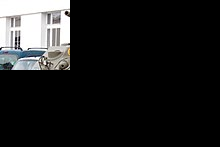
\includegraphics[width=0.14\textwidth]{img/czolg_masked_1.png}};
\node at (2,-1.5) {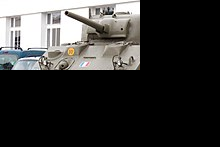
\includegraphics[width=0.14\textwidth]{img/czolg_masked_2.png}};
\node at (4,-1.5) {$\dots$};
\node at (6,-1.5) {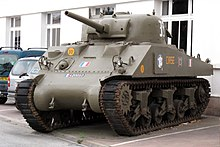
\includegraphics[width=0.14\textwidth]{img/czolg.jpg}};

\end{tikzpicture}
\end{center}
\end{minipage}
    \hrule
    \pause
    \begin{center}
    \textbf{Normalizing Flows} \\
    \begin{tikzpicture}
        \node[rand_var, inner sep=5pt] (z0) at (-1,0) {$z_0$};
        \node[rand_var, inner sep=5pt] (z1) at (1,0) {$z_1$};
        \node[rand_var, inner sep=5pt] (z2) at (3,0) {$z_2$};
        \node[inner sep=5pt] (dots) at (5,0) {$\ldots$};
        \node[rand_var, inner sep=5pt] (zk) at (7,0) {$z_k$};
        \draw[->] (z0) to node[above] {$f_1(z_0)$} (z1);
        \draw[->] (z1) to node[above] {$f_2(z_1)$} (z2);
        \draw[->] (z2) to node[above] {$f_3(z_2)$} (dots);
        \draw[->] (dots) to node[above] {$f_k(z_{k-1})$} (zk);
        % gaussian distribution and transformed ones
            \begin{scope}[shift={(-1,-0.75)},scale=0.075]
        \begin{axis}[
            anchor=center,
            domain=-3:3,
            samples=100,
            height=10cm,
            width=10cm,
            yticklabels={,,},
            xticklabels={,,},
            xmin=-3, xmax=3,
            ymin=0, ymax=0.5
        ]
        \addplot[smooth, very thick, blue] {1/sqrt(2*pi) * exp(-x^2/2)};
        \end{axis}
    \end{scope}
    % first trafo:
    \begin{scope}[shift={(1,-0.75)},scale=0.075]
        \begin{axis}[
            anchor=center,
            domain=-3:3,
            samples=100,
            height=10cm,
            width=10cm,
            yticklabels={,,},
            xticklabels={,,},
            xmin=-3, xmax=3,
            ymin=0, ymax=0.5
        ]
        \addplot[smooth, very thick, blue]  
        {0.5*(1/sqrt(0.5*2*pi) * exp(-(x+0.5)^2/(2*0.5^2))) 
        + 0.5*(1/sqrt(0.7*2*pi) * exp(-(x-1)^2/(2*0.7^2)))};
        \end{axis}
    \end{scope}
    % second trafo:
    \begin{scope}[shift={(3,-0.75)},scale=0.075]
        \begin{axis}[
            anchor=center,
            domain=-3:3,
            samples=100,
            height=10cm,
            width=10cm,
            yticklabels={,,},
            xticklabels={,,},
            xmin=-3, xmax=3,
            ymin=0, ymax=0.5
        ]
        \addplot[smooth, very thick, blue]  
        {0.3*(1/sqrt(0.3*2*pi) * exp(-(x+0.25)^2/(2*0.3^2))) 
        + 0.2*(1/sqrt(0.15*2*pi) * exp(-(x+1.15)^2/(2*0.15^2))) 
        + 0.5*(1/sqrt(0.7*2*pi) * exp(-(x-1)^2/(2*0.7^2)))};
        \end{axis}
    \end{scope}
    \node at (5,-0.75) {$\dots$};
   % final distribution:
    \begin{scope}[shift={(7,-0.75)},scale=0.075]
        \begin{axis}[
            anchor=center,
            domain=-3:3,
            samples=100,
            height=10cm,
            width=10cm,
            yticklabels={,,},
            xticklabels={,,},
            xmin=-3, xmax=3,
            ymin=0, ymax=0.5
        ]
        \addplot[smooth, very thick, blue] 
        {0.3*(1/sqrt(0.3*2*pi) * exp(-(x+0.25)^2/(2*0.3^2))) 
        + 0.2*(1/sqrt(0.15*2*pi) * exp(-(x+1.15)^2/(2*0.15^2))) 
        + 0.15*(1/sqrt(0.4*2*pi) * exp(-(x-2.1)^2/(2*0.4^2)))
        + 0.35*(1/sqrt(0.2*2*pi) * exp(-(x-0.9)^2/(2*0.2^2)))};
        \end{axis}
    \end{scope}
        \end{tikzpicture}
    \end{center}
    \hrule
    \pause
    \begin{center}
    \textbf{Diffusion Model} (a.k.a.\ Markovian Hierarchical Variational Autoencoder)
    % generate noisy images
%    \immediate\write18{python3 img/noise_image.py img/SuperMario.png img/SuperMario_noise_40.png 40}
%    \immediate\write18{python3 img/noise_image.py img/SuperMario.png img/SuperMario_noise_80.png 80}
%    \immediate\write18{python3 img/noise_image.py img/SuperMario.png img/SuperMario_noise_100.png 100}
    \begin{tikzpicture}
        \node[rand_var, inner sep=5pt] (x) at (-1,0) {$x$};
        \node[rand_var, inner sep=5pt] (z1) at (1,0) {$z_1$};
        \node[rand_var, inner sep=5pt] (z2) at (3,0) {$z_2$};
        \node[inner sep=5pt] (dots) at (5,0) {$\ldots$};
        \node[rand_var, inner sep=5pt] (zT) at (7,0) {$z_T$};
        \draw[->, bend left=45] (x) to node[above] {$q(z_1|x)$} (z1);
        \draw[->, bend left=45] (z1) to node[above] {$q(z_2|z_1)$} (z2);
        \draw[->, bend left=45] (z2) to node[above] {$q(z_3|z_2)$} (dots);
        \draw[->, bend left=45] (dots) to node[above] {$q(z_{T}|z_{T-1})$} (zT);
        \draw[->, bend left=45] (zT) to node[below] {$p(z_{T-1}|z_T)$} (dots);
        \draw[->, bend left=45] (dots) to node[below] {$p(z_2|z_3)$} (z2);
        \draw[->, bend left=45] (z2) to node[below] {$p(z_1|z_2)$} (z1);
        \draw[->, bend left=45] (z1) to node[below] {$p(x|z_1)$} (x);
        
        \node at (-1,-1) {\includegraphics[width=0.05\textwidth]{img/SuperMario.png}};
        \node at (1,-1) {\includegraphics[width=0.05\textwidth]{img/SuperMario_noise_40.png}};
        \node at (3,-1) {\includegraphics[width=0.05\textwidth]{img/SuperMario_noise_80.png}};
        \node at (5,-1) {$\dots$};
        \node at (7,-1) {\includegraphics[width=0.05\textwidth]{img/SuperMario_noise_100.png}};
        \end{tikzpicture}
    \end{center}
\end{frame}

\begin{frame}{Deep Learning vs.\ PML}
\begin{center}
\begin{tabular}{|>{\columncolor{gray!30}}p{0.15\textwidth}|p{0.33\textwidth}|p{0.33\textwidth}|}
    \hline
    \rowcolor{gray!30}
& \textbf{Deep Learning} & \textbf{Probabilistic Machine Learning} \\ \hline
\textbf{Goals} & Classification, feature learning, regression & Sampling, infering latent variables \\ \hline
\pause
\textbf{Vocabulary} & Neurons, activations, layers, $\ldots$ & Random variables, potentials \\ \hline
\pause
\textbf{Mathematical technique} & Differentiating & Sampling, marginalizing, differentiating \\ \hline
\pause
\textbf{Inference} & Simple forward pass & Monte-Carlo, belief propagation, message passing, linear programming, dynamic programming, $\ldots$ \\ \hline
\pause
\textbf{Learning} & Backprop \& gradient descent & MLE, EM, ELBO, $\ldots$ \\ \hline
\pause
\textbf{Impementation} & Many tricks to make it work & More standardized? \\ \hline
\end{tabular}
\pause
\vspace{0.1cm}

\textbf{Wisdom:} use DL + probabilistic techniques!\\
\vspace{0.2cm}
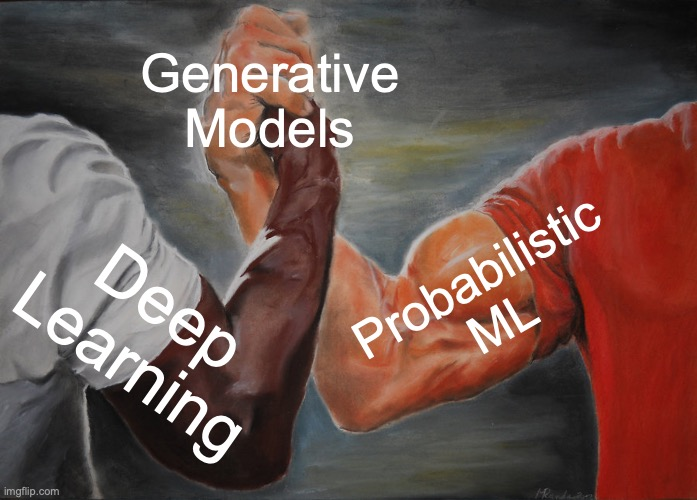
\includegraphics[width=0.3\textwidth]{img/dl+pml=generative.jpeg}\\
\end{center}
\end{frame}

\begin{frame}{PGM Lecture Overview}
\begin{minipage}{0.49\textwidth}
\begin{itemize}
    \item Bayesian (Directed) Graphical Models
    \begin{itemize}
    \item Conditional Independence, Factorization, Separation
    \end{itemize}
    \item Undirected (Markov) Graphical Models
    \item Inference in PGMs
    \begin{itemize}
        \item Exact
        \item Approximate: Monte-Carlo \& Variational
    \end{itemize}
    \item Learning PGMs
    \begin{itemize}
    \item MLE
    \item Expectation-Maximization
    \end{itemize}
\end{itemize}
\end{minipage}
\begin{minipage}{0.49\textwidth}
\begin{itemize}
    \item Autoregressive Models
    \item VAEs 
    \item Normalizing Flows
    \item Diffusion Models
\end{itemize}
\end{minipage}
\end{frame}
